\section{Networks}
\label{sec:api_networks}

% Networks are the final piece of the puzzle that makes up the Brel API.
% Together with resources and components, they are the parts of XBRL that are not yet covered by the OIM.
% Brel aims to give them the same treatment as the OIM parts of XBRL.
% This section will describe how Brel represents networks and their nodes.
Networks represent the final component essential to the Brel API, completing the framework alongside resources and components. 
These elements constitute parts of XBRL not yet encompassed by the OIM, 
but Brel seeks to integrate them with the same level of detail and organization.

At their core, networks are a collection of nodes.
Each node points to either a fact, a resource or a report element.
Nodes can have at most one parent node and an arbitrary number of child nodes.
The whole network can be represented simply by a list of root nodes.
These root have children, which have children, and so on.
Thus, the whole is accessible through the roots.

% Like other parts of Brel before them, networks implement a common interface.
% This time, there are two interfaces - \texttt{INetwork} and \texttt{INetworkNode}.
Consistent with previous Brel parts of the API, networks implement a common interface, 
in this case, two interfaces: \texttt{INetwork} and \texttt{INetworkNode}.


\begin{figure}[H]
    \centering
    \caption{UML diagram of the \texttt{INetwork} and \texttt{INetworkNode} interfaces}
    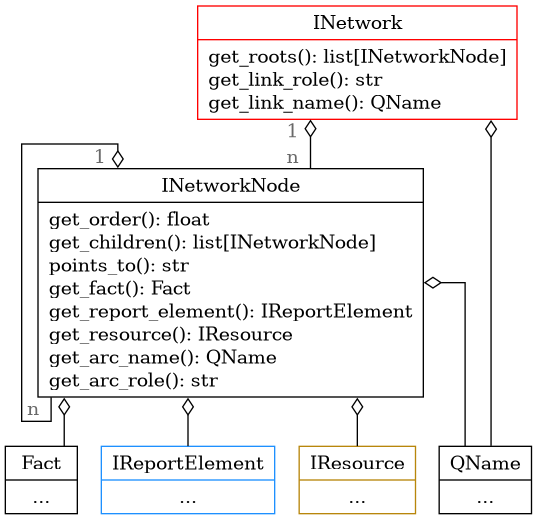
\includegraphics[width=0.5\textwidth]{images/brel_network_interfaces.png}
    \label{fig:brel_network_interfaces}
\end{figure}

\subsection{INetwork and INetworkNode}

The \texttt{INetwork} interface functions as a wrapper around a list of root nodes.
It provides a method for getting all root nodes, named \texttt{get\_roots}.

In addition to roots, \texttt{INetworkNode} provides access to both the link role and the link name 
of the underlying network with \texttt{get\_link\_role} and \texttt{get\_link\_name}.
These two methods expose the underlying XML structure of XBRL, raising the question of their inclusion in the Brel API.

% The reason is that they are useful for debugging.
% Networks are the part of XBRL where filers are most likely to make mistakes.
% Both the link role and the link name serve as sanity checks for filers and analysts alike.
% They might be removed from the API in the future, but for now they are useful for debugging.
The justification lies in their utility for debugging.
Errors in networks are common in XBRL submissions.
The link role and link name function as verification tools for both filers and analysts.
Although their presence in the API might be temporary, they currently serve a vital role in debugging.

% The \texttt{INetworkNode} interface also provides a method for getting all child nodes of a node, called \texttt{get\_children}.
% A node can not access its parent node directly, but since the graphs roots are accessible through the \texttt{INetwork} interface,
% the parent of a node can be found by traversing the graph from the roots.
Furthermore, the \texttt{INetworkNode} interface offers a way to obtain a node's child nodes via \texttt{get\_children}.
While direct access to a parent node is not available, one can identify a node's parent
by navigating from the graph's roots, provided by the \texttt{INetwork} interface.

% These two methods cover all of the functionality that is needed to traverse a network.
These functionalities suffice for navigating through a network.
% Subsequent methods address the retrieval of elements a node references.
% The subsequent methods are about getting the elements that a node points to.
The subsequent methods address the retrieval of elements that a node points to.

% Given a node can point to different types of elements, the \texttt{INetworkNode} interface provides the method \texttt{points\_to}.
Given the variety of elements a node can reference, the \texttt{INetworkNode} interface includes the \texttt{points\_to} method.
This method returns a string that indicates the type of element that the node points to.
The possible return values are \texttt{fact}, \texttt{resource} and \texttt{report element}.

% The interface also defines the methods \texttt{get\_fact}, \texttt{get\_resource} and \texttt{get\_report\_element},
Additionally, the interface defines getters named \texttt{get\_fact}, \texttt{get\_resource}, and \texttt{get\_report\_element}.
% which do exactly what their names suggest.
If the node does not point to the requested element, the methods raises an exception.

The methods \texttt{get\_arc\_role} and \texttt{get\_arc\_name} disclose diagnostic information about the network's underlying XML structure.
% Similar to the link role and link name, these methods expose the underlying XML structure of XBRL and are only used for debugging.

\subsection{Network Types}

As outlined in section \ref{sec:xbrl_networks}, XBRL features six different network types.
% All of them have their own Network- and Node-classes in Brel.
Each type is represented by its own Network and Node classes in Brel,
named to reflect the network type they represent, with the suffix \texttt{Network} or \texttt{NetworkNode}.
% The classes are named after the network type they represent, with the suffix \texttt{Network} or \texttt{NetworkNode}.
The table \ref{tab:network_types} lists the different network types and their corresponding classes.
% shows the different network types and their corresponding classes.

\begin{table}[H]
    \centering
    \caption{Network types and their corresponding classes}
    \begin{tabular}{|l|l|l|}
        \hline
        \textbf{Network type} & \textbf{Network class} & \textbf{Node class} \\ \hline
        Presentation          & \texttt{PresentationNetwork}          & \texttt{PresentationNetworkNode}          \\ \hline
        Calculation           & \texttt{CalculationNetwork}           & \texttt{CalculationNetworkNode}           \\ \hline
        Definition            & \texttt{DefinitionNetwork}            & \texttt{DefinitionNetworkNode}            \\ \hline
        Label                 & \texttt{LabelNetwork}                 & \texttt{LabelNetworkNode}                 \\ \hline
        Reference             & \texttt{ReferenceNetwork}             & \texttt{ReferenceNetworkNode}             \\ \hline
        Footnote              & \texttt{FootnoteNetwork}              & \texttt{FootnoteNetworkNode}              \\ \hline
    \end{tabular}
    \label{tab:network_types}
\end{table}

All of these classes implement the \texttt{INetwork} and \texttt{INetworkNode} interfaces without any modifications.
% Since the interfaces are so simple, yet gives access to all the information in the network,
Given the interfaces' simplicity and comprehensive access to network information,
% there is no need to change them for each network type.
alterations are unnecessary for each network type.
% The different semantic meanings of the networks can be expressed as helper function, which this chapter does not cover.
The unique semantic meanings of the networks are addressed through helper functions, which this chapter does not cover.
For completeness, the following diagrams show the inheritance structure of the network- and node-classes.

\begin{figure}[H]
    \centering
    \caption{UML diagram of the network classes}
    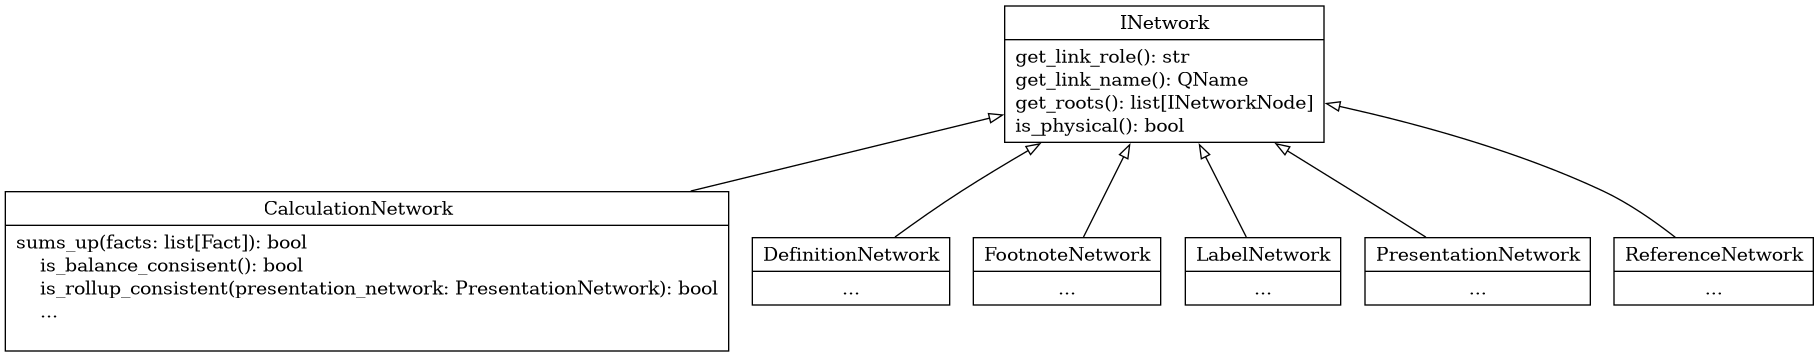
\includegraphics[width=\textwidth]{images/brel_network_classes.png}
    \label{fig:brel_network_classes}
\end{figure}

\begin{figure}[H]
    \centering
    \caption{UML diagram of the node classes}
    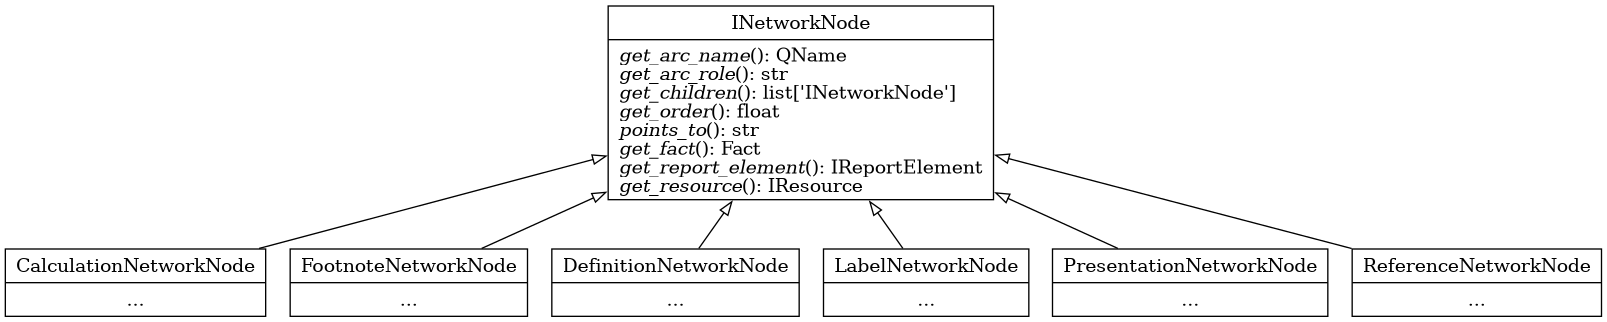
\includegraphics[width=\textwidth]{images/brel_network_node_classes.png}
    \label{fig:brel_network_node_classes}
\end{figure}

% With the network- and node-classes out of the way, Brel has covered all parts of XBRL it has set out to cover.
% The thing remaining with regards to the API is to see how the second half of this chapter answers research question \ref{RQ2}.
By addressing network- and node classes, Brel has successfully covered all aspects of XBRL it aimed to encompass.
What remains concerning the API is to explore how the latter section of this chapter addresses research question \ref{RQ2}.
